\documentclass{standalone}
\usepackage{tikz}
\usetikzlibrary{
  arrows,
  calc,
  decorations.pathmorphing,
  decorations.pathreplacing,
  decorations.markings,
  fadings,
  positioning,
  shapes,
  arrows.meta
}
\pgfdeclareradialshading{glow}{\pgfpoint{0cm}{0cm}}{
  color(0mm)=(white);
  color(5mm)=(white);
  color(9mm)=(black);
  color(10mm)=(black)
}

\begin{tikzfadingfrompicture}[name=glow fading]
  \shade [shading=glow] (0,0) circle (1);
\end{tikzfadingfrompicture}

\ifpdf
% Ensure reproducible output
\pdfinfoomitdate=1
\pdfsuppressptexinfo=-1
\pdftrailerid{}
\fi

\definecolor{atomblue}{rgb}{0,0,1}
\definecolor{atomorange}{rgb}{1,0.483,0}

\begin{document}

% Scale figure so that the text in the final plot is consistent with other figures
% note that the figure size needs to be scaled separately.
\begin{tikzpicture}[scale=1.27]
  \node at (-1.85, -0.5) {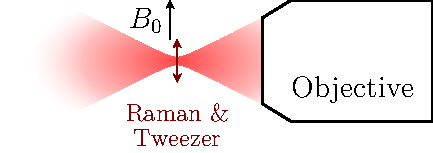
\includegraphics[width=1.7cm]{imgs/apparatus}};
  \node at (-2.5, 0.5) {\footnotesize (\textbf{A})};
  \node at (0.648, -0.8) {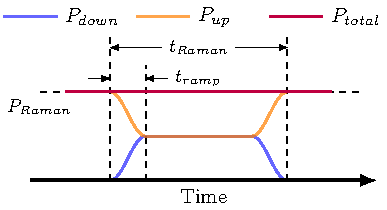
\includegraphics[width=5.0cm]{imgs/sequence}};
  \node at (-1.1, 0.5) {\footnotesize (\textbf{B})};
  \node at (0, -4.1) {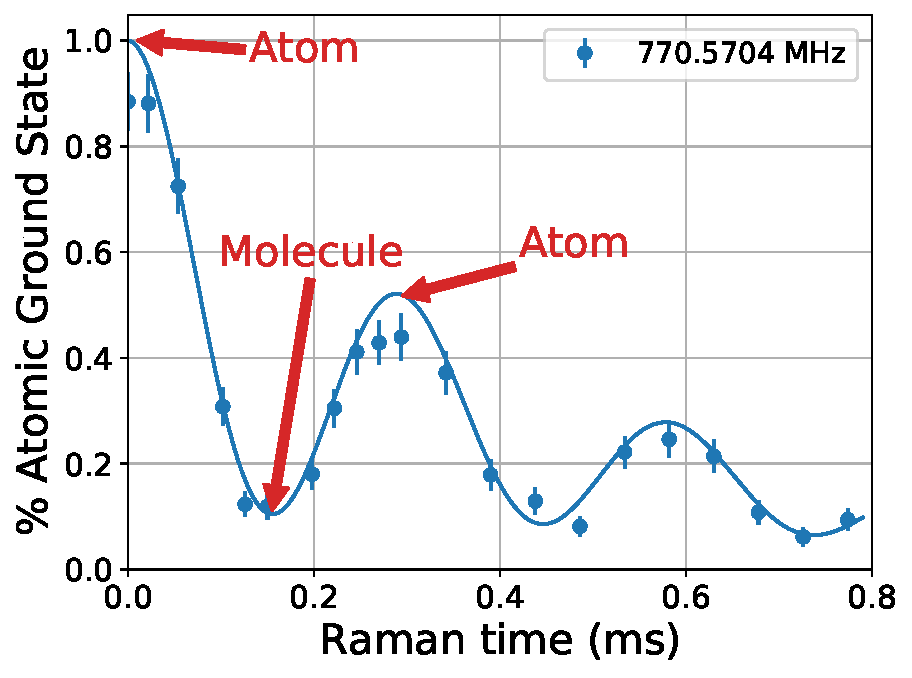
\includegraphics[width=6.75cm]{imgs/exp_data_norm_t.pdf}};
  \begin{scope}[shift={(-1.8, -2.35)}]
    \fill[atomblue] (0, 0.01) circle (0.075);
    \fill[atomorange] (0 + 0.317, -0.01) circle (0.05);
  \end{scope}
  \begin{scope}[shift={(-0.7, -3.9)}]
    \fill[atomblue] (0, 0.01) circle (0.075);
    \fill[atomorange] (0 + 0.317, -0.01) circle (0.05);
  \end{scope}
  \begin{scope}[shift={(-1.3, -5.5)}]
    \draw (0, 0.0) -- (0 + 0.317, 0.0);
    \fill[atomblue] (0, 0.0) circle (0.075);
    \fill[atomorange] (0 + 0.317, 0.0) circle (0.05);
  \end{scope}
  \node at (-2.15, -2.1) {\footnotesize (\textbf{C})};
  \node at (1.2, -3.48) {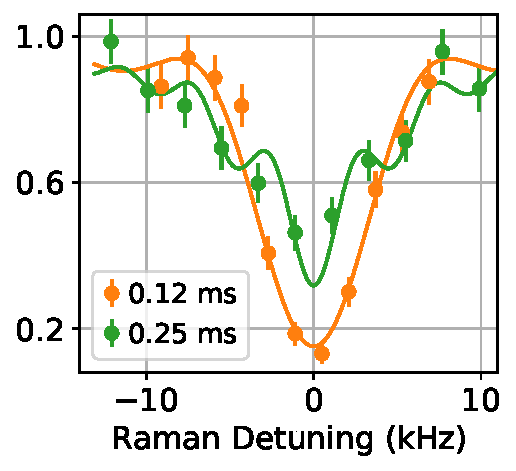
\includegraphics[width=3.4cm]{imgs/exp_data_norm_raman_det_inset.pdf}};
\end{tikzpicture}

\end{document}
